\documentclass[a4paper,12pt]{ETHexercise}
\usepackage{bbm}

\textheight24cm
\topmargin-2.5cm
\oddsidemargin+0cm
\textwidth16.3cm

\usepackage{amsmath}
\usepackage{amsfonts}
\usepackage{amssymb}
\usepackage{color}
\usepackage[latin1]{inputenc}
\usepackage{ifthen}
\usepackage{enumerate}
\usepackage{lastpage}
\usepackage{graphicx}
%\usepackage{subfigure}
\usepackage{subcaption}
\usepackage{bm}
\usepackage{tikz}
\usepackage{pgfplots}
\usepackage{float}
\usepackage{nicefrac}
\usepackage{epsfig}
\usepackage{etoolbox}
\usepackage{framed}
\usepackage{enumitem}
\usepackage{hyperref}
\usepackage{datetime}
\usepackage{url}
%\usepackage{algorithm}
\usepackage{svg}
\usepackage[ruled,vlined, linesnumbered]{algorithm2e}
\usepackage{setspace}
\usepackage[htt]{hyphenat}
\usepackage{qtree}
\usepackage{forest}
\usepackage{inconsolata} % for texttt{}


\usepackage[noend]{algpseudocode}
\algnewcommand{\parState}[1]{\State%
  \parbox[t]{\dimexpr\linewidth-\algmargin}{\strut\hangindent=\algorithmicindent \hangafter=1 #1\strut}}

\algrenewcommand\algorithmicindent{1.0em}%
\renewcommand\algorithmicdo{:}
\renewcommand\algorithmicthen{:}
%%%%% NEW MATH DEFINITIONS %%%%%

\usepackage{amsmath,amsfonts,bm}
\usepackage{xifthen}

% Added definitions

% Derivatev
\newcommand{\deriv}[3][]{
	\ifthenelse{\isempty{#1}}
	{\frac{\partial #2}{\partial #3}}
	{\frac{\partial^#1 #2}{\partial #3} }
}

% Mark sections of captions for referring to divisions of figures
\newcommand{\figleft}{{\em (Left)}}
\newcommand{\figcenter}{{\em (Center)}}
\newcommand{\figright}{{\em (Right)}}
\newcommand{\figtop}{{\em (Top)}}
\newcommand{\figbottom}{{\em (Bottom)}}
\newcommand{\captiona}{{\em (a)}}
\newcommand{\captionb}{{\em (b)}}
\newcommand{\captionc}{{\em (c)}}
\newcommand{\captiond}{{\em (d)}}

% Highlight a newly defined term
\newcommand{\newterm}[1]{{\bf #1}}


% Figure reference, lower-case.
\def\figref#1{figure~\ref{#1}}
% Figure reference, capital. For start of sentence
\def\Figref#1{Figure~\ref{#1}}
\def\twofigref#1#2{figures \ref{#1} and \ref{#2}}
\def\quadfigref#1#2#3#4{figures \ref{#1}, \ref{#2}, \ref{#3} and \ref{#4}}
% Section reference, lower-case.
\def\secref#1{section~\ref{#1}}
% Section reference, capital.
\def\Secref#1{Section~\ref{#1}}
% Reference to two sections.
\def\twosecrefs#1#2{sections \ref{#1} and \ref{#2}}
% Reference to three sections.
\def\secrefs#1#2#3{sections \ref{#1}, \ref{#2} and \ref{#3}}
% Reference to an equation, lower-case.
\def\eqref#1{equation~\ref{#1}}
% Reference to an equation, upper case
\def\Eqref#1{Equation~\ref{#1}}
% A raw reference to an equation---avoid using if possible
\def\plaineqref#1{\ref{#1}}
% Reference to a chapter, lower-case.
\def\chapref#1{chapter~\ref{#1}}
% Reference to an equation, upper case.
\def\Chapref#1{Chapter~\ref{#1}}
% Reference to a range of chapters
\def\rangechapref#1#2{chapters\ref{#1}--\ref{#2}}
% Reference to an algorithm, lower-case.
\def\algref#1{algorithm~\ref{#1}}
% Reference to an algorithm, upper case.
\def\Algref#1{Algorithm~\ref{#1}}
\def\twoalgref#1#2{algorithms \ref{#1} and \ref{#2}}
\def\Twoalgref#1#2{Algorithms \ref{#1} and \ref{#2}}
% Reference to a part, lower case
\def\partref#1{part~\ref{#1}}
% Reference to a part, upper case
\def\Partref#1{Part~\ref{#1}}
\def\twopartref#1#2{parts \ref{#1} and \ref{#2}}

\def\ceil#1{\lceil #1 \rceil}
\def\floor#1{\lfloor #1 \rfloor}
\def\1{\bm{1}}
\newcommand{\train}{\mathcal{D}}
\newcommand{\valid}{\mathcal{D_{\mathrm{valid}}}}
\newcommand{\test}{\mathcal{D_{\mathrm{test}}}}

\def\eps{{\epsilon}}


% Random variables
\def\reta{{\textnormal{$\eta$}}}
\def\ra{{\textnormal{a}}}
\def\rb{{\textnormal{b}}}
\def\rc{{\textnormal{c}}}
\def\rd{{\textnormal{d}}}
\def\re{{\textnormal{e}}}
\def\rf{{\textnormal{f}}}
\def\rg{{\textnormal{g}}}
\def\rh{{\textnormal{h}}}
\def\ri{{\textnormal{i}}}
\def\rj{{\textnormal{j}}}
\def\rk{{\textnormal{k}}}
\def\rl{{\textnormal{l}}}
% rm is already a command, just don't name any random variables m
\def\rn{{\textnormal{n}}}
\def\ro{{\textnormal{o}}}
\def\rp{{\textnormal{p}}}
\def\rq{{\textnormal{q}}}
\def\rr{{\textnormal{r}}}
\def\rs{{\textnormal{s}}}
\def\rt{{\textnormal{t}}}
\def\ru{{\textnormal{u}}}
\def\rv{{\textnormal{v}}}
\def\rw{{\textnormal{w}}}
\def\rx{{\textnormal{x}}}
\def\ry{{\textnormal{y}}}
\def\rz{{\textnormal{z}}}

% Random vectors
\def\rvepsilon{{\mathbf{\epsilon}}}
\def\rvtheta{{\mathbf{\theta}}}
\def\rva{{\mathbf{a}}}
\def\rvb{{\mathbf{b}}}
\def\rvc{{\mathbf{c}}}
\def\rvd{{\mathbf{d}}}
\def\rve{{\mathbf{e}}}
\def\rvf{{\mathbf{f}}}
\def\rvg{{\mathbf{g}}}
\def\rvh{{\mathbf{h}}}
\def\rvu{{\mathbf{i}}}
\def\rvj{{\mathbf{j}}}
\def\rvk{{\mathbf{k}}}
\def\rvl{{\mathbf{l}}}
\def\rvm{{\mathbf{m}}}
\def\rvn{{\mathbf{n}}}
\def\rvo{{\mathbf{o}}}
\def\rvp{{\mathbf{p}}}
\def\rvq{{\mathbf{q}}}
\def\rvr{{\mathbf{r}}}
\def\rvs{{\mathbf{s}}}
\def\rvt{{\mathbf{t}}}
\def\rvu{{\mathbf{u}}}
\def\rvv{{\mathbf{v}}}
\def\rvw{{\mathbf{w}}}
\def\rvx{{\mathbf{x}}}
\def\rvy{{\mathbf{y}}}
\def\rvz{{\mathbf{z}}}

% Elements of random vectors
\def\erva{{\textnormal{a}}}
\def\ervb{{\textnormal{b}}}
\def\ervc{{\textnormal{c}}}
\def\ervd{{\textnormal{d}}}
\def\erve{{\textnormal{e}}}
\def\ervf{{\textnormal{f}}}
\def\ervg{{\textnormal{g}}}
\def\ervh{{\textnormal{h}}}
\def\ervi{{\textnormal{i}}}
\def\ervj{{\textnormal{j}}}
\def\ervk{{\textnormal{k}}}
\def\ervl{{\textnormal{l}}}
\def\ervm{{\textnormal{m}}}
\def\ervn{{\textnormal{n}}}
\def\ervo{{\textnormal{o}}}
\def\ervp{{\textnormal{p}}}
\def\ervq{{\textnormal{q}}}
\def\ervr{{\textnormal{r}}}
\def\ervs{{\textnormal{s}}}
\def\ervt{{\textnormal{t}}}
\def\ervu{{\textnormal{u}}}
\def\ervv{{\textnormal{v}}}
\def\ervw{{\textnormal{w}}}
\def\ervx{{\textnormal{x}}}
\def\ervy{{\textnormal{y}}}
\def\ervz{{\textnormal{z}}}

% Random matrices
\def\rmA{{\mathbf{A}}}
\def\rmB{{\mathbf{B}}}
\def\rmC{{\mathbf{C}}}
\def\rmD{{\mathbf{D}}}
\def\rmE{{\mathbf{E}}}
\def\rmF{{\mathbf{F}}}
\def\rmG{{\mathbf{G}}}
\def\rmH{{\mathbf{H}}}
\def\rmI{{\mathbf{I}}}
\def\rmJ{{\mathbf{J}}}
\def\rmK{{\mathbf{K}}}
\def\rmL{{\mathbf{L}}}
\def\rmM{{\mathbf{M}}}
\def\rmN{{\mathbf{N}}}
\def\rmO{{\mathbf{O}}}
\def\rmP{{\mathbf{P}}}
\def\rmQ{{\mathbf{Q}}}
\def\rmR{{\mathbf{R}}}
\def\rmS{{\mathbf{S}}}
\def\rmT{{\mathbf{T}}}
\def\rmU{{\mathbf{U}}}
\def\rmV{{\mathbf{V}}}
\def\rmW{{\mathbf{W}}}
\def\rmX{{\mathbf{X}}}
\def\rmY{{\mathbf{Y}}}
\def\rmZ{{\mathbf{Z}}}

% Elements of random matrices
\def\ermA{{\textnormal{A}}}
\def\ermB{{\textnormal{B}}}
\def\ermC{{\textnormal{C}}}
\def\ermD{{\textnormal{D}}}
\def\ermE{{\textnormal{E}}}
\def\ermF{{\textnormal{F}}}
\def\ermG{{\textnormal{G}}}
\def\ermH{{\textnormal{H}}}
\def\ermI{{\textnormal{I}}}
\def\ermJ{{\textnormal{J}}}
\def\ermK{{\textnormal{K}}}
\def\ermL{{\textnormal{L}}}
\def\ermM{{\textnormal{M}}}
\def\ermN{{\textnormal{N}}}
\def\ermO{{\textnormal{O}}}
\def\ermP{{\textnormal{P}}}
\def\ermQ{{\textnormal{Q}}}
\def\ermR{{\textnormal{R}}}
\def\ermS{{\textnormal{S}}}
\def\ermT{{\textnormal{T}}}
\def\ermU{{\textnormal{U}}}
\def\ermV{{\textnormal{V}}}
\def\ermW{{\textnormal{W}}}
\def\ermX{{\textnormal{X}}}
\def\ermY{{\textnormal{Y}}}
\def\ermZ{{\textnormal{Z}}}

% Vectors
\def\vzero{{\bm{0}}}
\def\vone{{\bm{1}}}
\def\vmu{{\bm{\mu}}}
\def\vtheta{{\bm{\theta}}}
\def\va{{\bm{a}}}
\def\vb{{\bm{b}}}
\def\vc{{\bm{c}}}
\def\vd{{\bm{d}}}
\def\ve{{\bm{e}}}
\def\vf{{\bm{f}}}
\def\vg{{\bm{g}}}
\def\vh{{\bm{h}}}
\def\vi{{\bm{i}}}
\def\vj{{\bm{j}}}
\def\vk{{\bm{k}}}
\def\vl{{\bm{l}}}
\def\vm{{\bm{m}}}
\def\vn{{\bm{n}}}
\def\vo{{\bm{o}}}
\def\vp{{\bm{p}}}
\def\vq{{\bm{q}}}
\def\vr{{\bm{r}}}
\def\vs{{\bm{s}}}
\def\vt{{\bm{t}}}
\def\vu{{\bm{u}}}
\def\vv{{\bm{v}}}
\def\vw{{\bm{w}}}
\def\vx{{\bm{x}}}
\def\vy{{\bm{y}}}
\def\vz{{\bm{z}}}

% Elements of vectors
\def\evalpha{{\alpha}}
\def\evbeta{{\beta}}
\def\evepsilon{{\epsilon}}
\def\evlambda{{\lambda}}
\def\evomega{{\omega}}
\def\evmu{{\mu}}
\def\evpsi{{\psi}}
\def\evsigma{{\sigma}}
\def\evtheta{{\theta}}
\def\eva{{a}}
\def\evb{{b}}
\def\evc{{c}}
\def\evd{{d}}
\def\eve{{e}}
\def\evf{{f}}
\def\evg{{g}}
\def\evh{{h}}
\def\evi{{i}}
\def\evj{{j}}
\def\evk{{k}}
\def\evl{{l}}
\def\evm{{m}}
\def\evn{{n}}
\def\evo{{o}}
\def\evp{{p}}
\def\evq{{q}}
\def\evr{{r}}
\def\evs{{s}}
\def\evt{{t}}
\def\evu{{u}}
\def\evv{{v}}
\def\evw{{w}}
\def\evx{{x}}
\def\evy{{y}}
\def\evz{{z}}

% Matrix
\def\mA{{\bm{A}}}
\def\mB{{\bm{B}}}
\def\mC{{\bm{C}}}
\def\mD{{\bm{D}}}
\def\mE{{\bm{E}}}
\def\mF{{\bm{F}}}
\def\mG{{\bm{G}}}
\def\mH{{\bm{H}}}
\def\mI{{\bm{I}}}
\def\mJ{{\bm{J}}}
\def\mK{{\bm{K}}}
\def\mL{{\bm{L}}}
\def\mM{{\bm{M}}}
\def\mN{{\bm{N}}}
\def\mO{{\bm{O}}}
\def\mP{{\bm{P}}}
\def\mQ{{\bm{Q}}}
\def\mR{{\bm{R}}}
\def\mS{{\bm{S}}}
\def\mT{{\bm{T}}}
\def\mU{{\bm{U}}}
\def\mV{{\bm{V}}}
\def\mW{{\bm{W}}}
\def\mX{{\bm{X}}}
\def\mY{{\bm{Y}}}
\def\mZ{{\bm{Z}}}
\def\mBeta{{\bm{\beta}}}
\def\mPhi{{\bm{\Phi}}}
\def\mLambda{{\bm{\Lambda}}}
\def\mSigma{{\bm{\Sigma}}}

% Tensor
\DeclareMathAlphabet{\mathsfit}{\encodingdefault}{\sfdefault}{m}{sl}
\SetMathAlphabet{\mathsfit}{bold}{\encodingdefault}{\sfdefault}{bx}{n}
\newcommand{\tens}[1]{\bm{\mathsfit{#1}}}
\def\tA{{\tens{A}}}
\def\tB{{\tens{B}}}
\def\tC{{\tens{C}}}
\def\tD{{\tens{D}}}
\def\tE{{\tens{E}}}
\def\tF{{\tens{F}}}
\def\tG{{\tens{G}}}
\def\tH{{\tens{H}}}
\def\tI{{\tens{I}}}
\def\tJ{{\tens{J}}}
\def\tK{{\tens{K}}}
\def\tL{{\tens{L}}}
\def\tM{{\tens{M}}}
\def\tN{{\tens{N}}}
\def\tO{{\tens{O}}}
\def\tP{{\tens{P}}}
\def\tQ{{\tens{Q}}}
\def\tR{{\tens{R}}}
\def\tS{{\tens{S}}}
\def\tT{{\tens{T}}}
\def\tU{{\tens{U}}}
\def\tV{{\tens{V}}}
\def\tW{{\tens{W}}}
\def\tX{{\tens{X}}}
\def\tY{{\tens{Y}}}
\def\tZ{{\tens{Z}}}


% Graph
\def\gA{{\mathcal{A}}}
\def\gB{{\mathcal{B}}}
\def\gC{{\mathcal{C}}}
\def\gD{{\mathcal{D}}}
\def\gE{{\mathcal{E}}}
\def\gF{{\mathcal{F}}}
\def\gG{{\mathcal{G}}}
\def\gH{{\mathcal{H}}}
\def\gI{{\mathcal{I}}}
\def\gJ{{\mathcal{J}}}
\def\gK{{\mathcal{K}}}
\def\gL{{\mathcal{L}}}
\def\gM{{\mathcal{M}}}
\def\gN{{\mathcal{N}}}
\def\gO{{\mathcal{O}}}
\def\gP{{\mathcal{P}}}
\def\gQ{{\mathcal{Q}}}
\def\gR{{\mathcal{R}}}
\def\gS{{\mathcal{S}}}
\def\gT{{\mathcal{T}}}
\def\gU{{\mathcal{U}}}
\def\gV{{\mathcal{V}}}
\def\gW{{\mathcal{W}}}
\def\gX{{\mathcal{X}}}
\def\gY{{\mathcal{Y}}}
\def\gZ{{\mathcal{Z}}}

% Sets
\def\sA{{\mathbb{A}}}
\def\sB{{\mathbb{B}}}
\def\sC{{\mathbb{C}}}
\def\sD{{\mathbb{D}}}
% Don't use a set called E, because this would be the same as our symbol
% for expectation.
\def\sF{{\mathbb{F}}}
\def\sG{{\mathbb{G}}}
\def\sH{{\mathbb{H}}}
\def\sI{{\mathbb{I}}}
\def\sJ{{\mathbb{J}}}
\def\sK{{\mathbb{K}}}
\def\sL{{\mathbb{L}}}
\def\sM{{\mathbb{M}}}
\def\sN{{\mathbb{N}}}
\def\sO{{\mathbb{O}}}
\def\sP{{\mathbb{P}}}
\def\sQ{{\mathbb{Q}}}
\def\sR{{\mathbb{R}}}
\def\sS{{\mathbb{S}}}
\def\sT{{\mathbb{T}}}
\def\sU{{\mathbb{U}}}
\def\sV{{\mathbb{V}}}
\def\sW{{\mathbb{W}}}
\def\sX{{\mathbb{X}}}
\def\sY{{\mathbb{Y}}}
\def\sZ{{\mathbb{Z}}}

% Entries of a matrix
\def\emLambda{{\Lambda}}
\def\emA{{A}}
\def\emB{{B}}
\def\emC{{C}}
\def\emD{{D}}
\def\emE{{E}}
\def\emF{{F}}
\def\emG{{G}}
\def\emH{{H}}
\def\emI{{I}}
\def\emJ{{J}}
\def\emK{{K}}
\def\emL{{L}}
\def\emM{{M}}
\def\emN{{N}}
\def\emO{{O}}
\def\emP{{P}}
\def\emQ{{Q}}
\def\emR{{R}}
\def\emS{{S}}
\def\emT{{T}}
\def\emU{{U}}
\def\emV{{V}}
\def\emW{{W}}
\def\emX{{X}}
\def\emY{{Y}}
\def\emZ{{Z}}
\def\emSigma{{\Sigma}}

% entries of a tensor
% Same font as tensor, without \bm wrapper
\newcommand{\etens}[1]{\mathsfit{#1}}
\def\etLambda{{\etens{\Lambda}}}
\def\etA{{\etens{A}}}
\def\etB{{\etens{B}}}
\def\etC{{\etens{C}}}
\def\etD{{\etens{D}}}
\def\etE{{\etens{E}}}
\def\etF{{\etens{F}}}
\def\etG{{\etens{G}}}
\def\etH{{\etens{H}}}
\def\etI{{\etens{I}}}
\def\etJ{{\etens{J}}}
\def\etK{{\etens{K}}}
\def\etL{{\etens{L}}}
\def\etM{{\etens{M}}}
\def\etN{{\etens{N}}}
\def\etO{{\etens{O}}}
\def\etP{{\etens{P}}}
\def\etQ{{\etens{Q}}}
\def\etR{{\etens{R}}}
\def\etS{{\etens{S}}}
\def\etT{{\etens{T}}}
\def\etU{{\etens{U}}}
\def\etV{{\etens{V}}}
\def\etW{{\etens{W}}}
\def\etX{{\etens{X}}}
\def\etY{{\etens{Y}}}
\def\etZ{{\etens{Z}}}

% The true underlying data generating distribution
\newcommand{\pdata}{p_{\rm{data}}}
% The empirical distribution defined by the training set
\newcommand{\ptrain}{\hat{p}_{\rm{data}}}
\newcommand{\Ptrain}{\hat{P}_{\rm{data}}}
% The model distribution
\newcommand{\pmodel}{p_{\rm{model}}}
\newcommand{\Pmodel}{P_{\rm{model}}}
\newcommand{\ptildemodel}{\tilde{p}_{\rm{model}}}
% Stochastic autoencoder distributions
\newcommand{\pencode}{p_{\rm{encoder}}}
\newcommand{\pdecode}{p_{\rm{decoder}}}
\newcommand{\precons}{p_{\rm{reconstruct}}}

\newcommand{\laplace}{\mathrm{Laplace}} % Laplace distribution

\newcommand{\E}{\mathbb{E}}
\newcommand{\Ls}{\mathcal{L}}
\newcommand{\R}{\mathbb{R}}
\newcommand{\emp}{\tilde{p}}
\newcommand{\lr}{\alpha}
\newcommand{\reg}{\lambda}
\newcommand{\rect}{\mathrm{rectifier}}
\newcommand{\softmax}{\mathrm{softmax}}
\newcommand{\sigmoid}{\sigma}
\newcommand{\softplus}{\zeta}
\newcommand{\KL}{D_{\mathrm{KL}}}
\newcommand{\Var}{\mathrm{Var}}
\newcommand{\standarderror}{\mathrm{SE}}
\newcommand{\Cov}{\mathrm{Cov}}
% Wolfram Mathworld says $L^2$ is for function spaces and $\ell^2$ is for vectors
% But then they seem to use $L^2$ for vectors throughout the site, and so does
% wikipedia.
\newcommand{\normlzero}{L^0}
\newcommand{\normlone}{L^1}
\newcommand{\normltwo}{L^2}
\newcommand{\normlp}{L^p}
\newcommand{\normmax}{L^\infty}

\newcommand{\parents}{Pa} % See usage in notation.tex. Chosen to match Daphne's book.

\DeclareMathOperator*{\argmax}{arg\,max}
\DeclareMathOperator*{\argmin}{arg\,min}

\DeclareMathOperator{\sign}{sign}
\DeclareMathOperator{\Tr}{Tr}
\let\ab\allowbreak

%\newcommand{\linetofill}{\ \\\hphantom{\hspace{0mm}}\hrulefill\ \\}
\newcommand{\linetofill}{\ \\\hphantom{\hspace{0mm}}\dotfill\ \\}
\newcommand{\vlinetofill}[1]{\\\rule{#1 mm}{0.1mm}\ \\}
\newcommand{\cbox}{
  \setlength{\unitlength}{1pt}
  \begin{picture}(10,10)
    \put(0,0){\line(1,0){8}} \put(0,8){\line(1,0){8}}
    \put(0,0){\line(0,1){8}} \put(8,0){\line(0,1){8}}
  \end{picture}
}
\newcommand{\bigcbox}{
  \setlength{\unitlength}{3pt}
  \begin{picture}(10,10)(1,1)
    \put(0,0){\line(1,0){8}} \put(0,8){\line(1,0){8}}
    \put(0,0){\line(0,1){8}} \put(8,0){\line(0,1){8}}
  \end{picture}
}
% points and boxes on the right
\newcommand{\points}[1]{
  \ \\[-5mm]
  \hphantom{\ }\hfill\textbf{#1 pts \bigcbox \hspace{-6mm}}
  \vspace{5mm}
}
% multiple choice checkboxes
%\newcommand{\boxt}{\hspace*{2em} $[~~]$ \textsf{True}}
%\newcommand{\boxf}{\hspace*{2em} $[~~]$ \textsf{False}}
\newcommand{\boxt}{\hspace*{2em} $\square$ \textsf{True}}
\newcommand{\boxf}{\hspace*{2em} $\square$ \textsf{False}}
\newcommand{\justif}{\textsf{Justification}:  \rule{0ex}{2em}\dotfill\\\rule{0ex}{2em}\dotfill}
\newcommand{\checkboxWithJustification}{\boxt \boxf\\ \justif\\}
\newcommand{\checkbox}{\boxt \boxf}
\usepackage{tikz}
\usepackage{xcolor}
\usepackage{amssymb}
\usepackage{amsmath}
\usepackage{amsthm}
\usepackage{pgfplots}
\pgfmathdeclarefunction{gauss}{2}{%
  \pgfmathparse{1/(#2*sqrt(2*pi))*exp(-((x-#1)^2)/(2*#2^2))}%
}
\renewcommand{\S}{{\cal S}}
\usepackage{pgfplots}
\pgfplotsset{compat=newest}
\pgfplotsset{small, every non boxed x axis/.append style={x axis line style=-},
  every non boxed y axis/.append style={y axis line style=-}}

\newcommand{\timestamp}{\ddmmyyyydate\today \,\,- \currenttime h}
%%% Local Variables:
%%% mode: latex
%%% TeX-master: "exam"
%%% End:

% Numbers
\usepackage[group-separator={,}]{siunitx}

\usepackage{cleveref}
\crefname{section}{\S}{\S\S}
\Crefname{section}{\S}{\S\S}
\crefname{table}{Tab.}{}
\crefname{figure}{Fig.}{}
\crefname{algorithm}{Algorithm}{}
\crefname{equation}{eq.}{}
\crefname{appendix}{App.}{}
\crefname{thm}{Theorem}{}
\crefname{prop}{Proposition}{}
\crefname{cor}{Corollary}{}
\crefname{observation}{Observation}{}
\crefname{assumption}{Assumption}{}
\crefformat{section}{\S#2#1#3}

\usepackage{multirow}
\title{NLP Assignment}
\begin{document}
\setserie{1}


\newcommand{\pair}[2]{{\langle #1 , #2 \rangle}}
\newcommand{\score}[2]{\text{score}_{\theta}(\langle #1, #2 \rangle, \boldsymbol{w})}
\newcommand{\sscore}[1]{\text{score}_{\theta}(#1, \boldsymbol{w})}

\lectureheader{Prof. Ryan Cotterell}
{}
{\Large Natural Language Processing}{Fall 2022}
\begin{center}
	{\Huge Simon Wachter: Assignment 2}\\
	\quad\newline
	siwachte@ethz.ch, 19-920-198\\
	\quad\newline
	\timestamp
\end{center}

\begin{question}\\
	\begin{subquestion}
		Prove that the expectation semiring satisfies the semiring axioms:\\
		\begin{itemize}
			\item  $(\R \times \R, \oplus, \mathbf{0})$ must be a commutative monoid with identity element $\mathbf{0}$:
			      \begin{align}
				      \left(\pair{x}{y} \oplus \pair{x'}{y'}\right) \oplus \pair{x''}{y''} & =       \pair{x + x'}{y + y'}      \oplus \pair{x''}{y''}              \\
				                                                                           & = \pair{x + x' + x''}{y + y' + y''}                                    \\
				                                                                           & = \pair{x}{y} \oplus \pair{x' + x''}{y' + y''}                         \\
				                                                                           & = \pair{x}{y} \oplus \left(\pair{x'}{y'} \oplus \pair{x''}{y''}\right)
			      \end{align}
			      \begin{align}
				      \mathbf{0} + \pair{x}{y} & = \pair{0}{0} \oplus \pair{x}{y} \\
				                               & = \pair{0 + x}{0 + y}            \\
				                               & = \pair{x}{y}                    \\
				                               & = \pair{x + 0}{y + 0}            \\
				                               & = \pair{x}{y} + \mathbf{0}
			      \end{align}
			      \begin{align}
				      \pair{x}{y} + \pair{x'}{y'} & = \pair{x + x'}{y + y'}       \\
				                                  & = \pair{x' + x}{y' + y}       \\
				                                  & = \pair{x'}{y'} + \pair{x}{y}
			      \end{align}
			\item $(\R \times \R, \otimes, \mathbf{1})$ must be a monoid with identity element $\mathbf{1}$:
			      \begin{align}
				      \left(\pair{x}{y} \otimes \pair{x'}{y'} \right) \otimes \pair{x''}{y''} & = \pair{x \cdot x'}{x \cdot y' + y \cdot x'} \otimes \pair{x''}{y''}                              \\
				                                                                              & = \pair{x \cdot x' \cdot x''}{x \cdot x' \cdot y'' + (x \cdot y' + y \cdot x') \cdot x''}         \\
				                                                                              & = \pair{x \cdot x' \cdot x''}{x \cdot x' \cdot y'' + x \cdot y' \cdot x'' + y \cdot x' \cdot x''} \\
				                                                                              & = \pair{x}{y} \otimes \pair{x' \cdot x''}{x' \cdot y'' + y' \cdot x''}                            \\
				                                                                              & = \pair{x}{y} \otimes \left(\pair{x'}{y'} \otimes \pair{x''}{y''}\right)
			      \end{align}
			      \begin{align}
				      \mathbf{1} \otimes \pair{x}{y} & = \pair{1}{0} \otimes \pair{x}{y} \\
				                                     & = \pair{1 \cdot x}{1 \cdot y}     \\
				                                     & = \pair{x}{y}                     \\
				                                     & = \pair{x \cdot 1}{y \cdot 1}     \\
				                                     & = \pair{x}{y} \otimes \mathbf{1}
			      \end{align}
			\item Multiplication left and right distributes over addition:
			      \begin{align}
				      \pair{x}{y} \otimes \left(\pair{x'}{y'} \oplus \pair{x''}{y''}\right) & = \pair{x}{y} \otimes \pair{x' + x''}{y' + y''}                                                          \\
				                                                                            & = \pair{x \cdot x' + x \cdot x''}{x \cdot y' + x \cdot y'' + y \cdot x' + y \cdot x''}                   \\
				                                                                            & = \pair{x \cdot x'}{x \cdot y' + y \cdot x'} \oplus \pair{x \cdot x''}{x \cdot y'' + y \cdot x''}        \\
				                                                                            & = \left(\pair{x}{y} \otimes \pair{x'}{y'}\right) \oplus \left(\pair{x}{y} \otimes \pair{x''}{y''}\right)
			      \end{align}
			      \begin{align}
				      \left(\pair{x}{y} \oplus \pair{x'}{y'}\right) \otimes \pair{x''}{y''} & = \pair{x + x'}{y + y'} \otimes \pair{x''}{y''}                                                              \\
				                                                                            & = \pair{x \cdot x'' + x' \cdot x''}{x \cdot y'' + x' \cdot y'' + y \cdot x'' + y' \cdot x''}                 \\
				                                                                            & = \pair{x \cdot x''}{x \cdot y'' + y \cdot x''} \oplus \pair{x' \cdot x''}{x' \cdot y'' + y' \cdot x''}      \\
				                                                                            & = \left(\pair{x}{y} \otimes \pair{x''}{y''}\right) \oplus \left(\pair{x'}{y'} \otimes \pair{x''}{y''}\right)
			      \end{align}
			\item Multiplication by $\mathbf{0}$ annihilates $\R \times \R$:
			      \begin{align}
				      \mathbf{0} \otimes \pair{x}{y} & = \pair{0}{0} \otimes \pair{x}{y}       \\
				                                     & = \pair{0 \cdot x}{0 \cdot y}           \\
				                                     & = \pair{0}{0}                           \\    &= \mathbf{0}         \\
				                                     & = \pair{0}{0}                           \\
				                                     & = \pair{x \cdot 0}{y \cdot 0}           \\
				                                     & =       \pair{x}{y} \otimes \pair{0}{0} \\
				                                     & = \pair{x}{y} \otimes \mathbf{0}
			      \end{align}
		\end{itemize}
	\end{subquestion}
	\begin{subquestion}
		Our initial graph looks like \cref{figure:graph}.
		\begin{figure}[H]
			\centering
			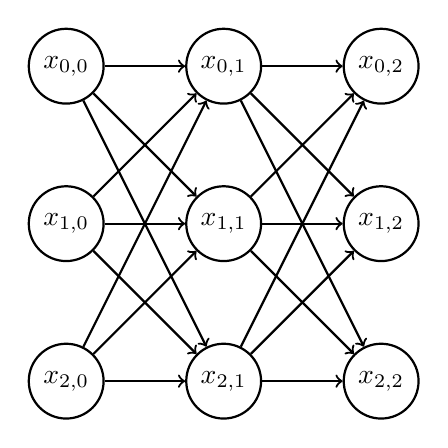
\begin{tikzpicture}[node distance={20mm}, thick, main/.style = {draw, circle}]
				\node[main] (0) {$x_{0,0}$};
				\node[main] (1) [below of=0]{$x_{1,0}$};
				\node[main] (2) [below of=1]{$x_{2,0}$};

				\node[main] (3) [right of=0]{$x_{0,1}$};
				\node[main] (4) [below of=3]{$x_{1,1}$};
				\node[main] (5) [below of=4]{$x_{2,1}$};

				\node[main] (6) [right of=3]{$x_{0,2}$};
				\node[main] (7) [below of=6]{$x_{1,2}$};
				\node[main] (8) [below of=7]{$x_{2,2}$};

				\draw[->] (0) -- (3);
				\draw[->] (0) -- (4);
				\draw[->] (0) -- (5);

				\draw[->] (1) -- (3);
				\draw[->] (1) -- (4);
				\draw[->] (1) -- (5);

				\draw[->] (2) -- (3);
				\draw[->] (2) -- (4);
				\draw[->] (2) -- (5);

				\draw[->] (3) -- (6);
				\draw[->] (3) -- (7);
				\draw[->] (3) -- (8);

				\draw[->] (4) -- (6);
				\draw[->] (4) -- (7);
				\draw[->] (4) -- (8);

				\draw[->] (5) -- (6);
				\draw[->] (5) -- (7);
				\draw[->] (5) -- (8);

			\end{tikzpicture}
			\caption[]{The initial graph}
			\label{figure:graph}
		\end{figure}
		Where the columns represent the words in $\mathbf{w}$ and the rows represent different tags.
		We use the algorithm from the script:\\
		\begin{algorithm}[H]
			\SetAlgoLined
			\caption{Forward pass}
			\label{algorithm:forward}
			$\beta(\mathbf{w}, t_0) = 1$\\
			\For{$n = 1 \to N$}{
				$\beta(\mathbf{w}, t_n) = \sum_{t_{n-1} \in \mathcal{T}} \exp(\score{\langle t_{n-1}}{t_n\rangle}) \otimes \beta(\mathbf{w}, t_{n-1})$
			}
		\end{algorithm}
		When we now lift the CRF into the expectation semiring, the forward propagation algorithm changes to:\\
		\begin{algorithm}[H]
			\SetAlgoLined
			\caption{Forward pass}
			\label{algorithm:forward_semi}
			$\beta(\mathbf{w}, t_0) = \langle 1, 0 \rangle$\\
			\For{$n = 1 \to N$}{
				$\beta(\mathbf{w}, t_n) = \oplus_{t_{n-1} \in \mathcal{T}} \langle w, -w \log w \rangle \otimes \beta(\mathbf{w}, t_{n-1})$
			}
		\end{algorithm}
		Where $w = \exp(\score{\langle t_n}{t_{n+1}\rangle})$.\\
		The output of the forward algorithm lifted into the semiring will yield:\\
		\begin{align}
			\bigoplus_{t_{1:N} \in T^{n}} \overset{N}{\bigotimes_{n=1}} \langle w, -w \log w \rangle
		\end{align}
		We want to show that the result of the forward propagation lifted in the semiring is the same as the unnormalized Entropy:
		\begin{align}
			H_u(T_{w}) & = -\sum_{\mathbf{t} \in \mathcal{T}^N} \exp(score_{\boldsymbol{\theta}} (\mathbf{t},\boldsymbol{w})) score_{\boldsymbol{\theta}} (\mathbf{t},\boldsymbol{w}) \label{eq:1b_to_show} \\
		\end{align}
		We show this by induction. Starting with the base case where $N = 1$:\\
		\begin{align}
			\bigoplus_{t_{1} \in T^{1}} \overset{1}{\bigotimes_{n=1}} \langle w, -w \log w \rangle & = \bigoplus_{t_{1} \in T^{1}} \langle \exp(\score{t_0}{t_1}),                     \\
			                                                                                       & \qquad -\exp(\score{t_0}{t_1}) \log(\exp(\score{t_0}{t_1})) \rangle               \\
			                                                                                       & = \bigoplus_{t \in T} \biggl< \exp(\sscore{t}),                         \nonumber \\
			                                                                                       & \qquad  -\exp(\sscore{t}) \log(\exp(\sscore{t})) \biggr>                          \\
			                                                                                       & = \biggl< \sum_{t \in T} \exp(\sscore{t}),                              \nonumber \\
			                                                                                       & \qquad -\sum_{t \in T} \exp(\sscore{t}) \log(\exp(\sscore{t})) \biggr>
		\end{align}
		Our induction hypothesis is the following:\\
		\begin{align}
			\bigoplus_{t_{1:i} \in T^{i}} \overset{i}{\bigotimes_{n=1}} \langle w, -w \log w \rangle = \left\langle \sum_{t \in T^{i}} \exp(\sscore{t}), -\sum_{t \in T^{i}} \exp(\sscore{t}) \log(\exp(\sscore{t})) \right\rangle
		\end{align}
		Meaning we assume that $\beta(\mathbf{w}, t_i)$ corresponds to the unnormalized entropy of all sequences of lenght $i$.\\
		Now we proceed with the induction step, where $i \rightarrow i + 1$:\\
		\begin{align}
			 & \bigoplus_{t_{1:i+1} \in T^{i+1}} \overset{i+1}{\bigotimes_{n=1}} \langle w, -w \log w \rangle \nonumber                                                                       \\ & = \bigoplus_{t_{1:i+1} \in T}  \left( \bigoplus_{t_{1:i} \in T^{i}} \overset{i}{\bigotimes_{n=1}} \langle w, -w \log w \rangle \right) \otimes \langle w, -w \log(w) \rangle \\
			 & \overset{\text{I.H.}}{=} \bigoplus_{t_{1:i+1} \in T} \left\langle \sum_{t \in T^{i}} \exp(\sscore{t}), -\sum_{t \in T^{i}} \exp(\sscore(t)) \sscore{t} \right\rangle \nonumber \\
			 & \otimes \left\langle \exp(\score{t_i}{t_{i+1}}), -\exp(\score{t_i}{t_{i+1}}) \score{t_i}{t_{i+1}}\right\rangle \label{eq:after_ih}
		\end{align}
		We will now analyze both parts of the semiring separately:
		\begin{align}
			 & \left(\sum_{t \in T^{i}} \exp(\sscore{t}) \right) \exp(\score{t_i}{t_{i+1}})                \\
			 & = \sum_{t \in T^{i}} \exp(\sscore{t}) + \score{t_i}{t_{i+1}}               \label{eq:semil}
		\end{align}
		And the second part:
		\begin{align}
			 & \left( \sum_{t \in T^{i}} \exp(\sscore{t}) \right) -\exp(\score{t_i}{t_{i+1}}) \score{t_i}{t_{i+1}} \nonumber                   \\
			 & \quad + \left( -\sum_{t \in T^{i}} \exp(\sscore(t)) \sscore{t} \right) \exp(\score{t_i}{t_{i+1}})                               \\
			 & = -\sum_{t \in T^{i}} \exp(\sscore{t} + \score{t_i}{t_{i+1}}) \score{t_i}{t_{i+1}} \nonumber                                    \\
			 & \quad -\left( \sum_{t \in T^{i}} \exp(\sscore(t)) \sscore{t} \right) \exp(\score{t_i}{t_{i+1}})                                 \\
			 & = -\sum_{t \in T^{i}} \exp(\sscore{t} + \score{t_i}{t_{i+1}}) \score{t_i}{t_{i+1}} \nonumber                                    \\
			 & \quad - \sum_{t \in T^{i}} \exp(\sscore{t} + \score{t_i}{t_{i+1}}) \sscore{t}                                                   \\
			 & = -\sum_{t \in T^{i}} \exp(\sscore{t} + \score{t_i}{t_{i+1}}) \left( \sscore{t} + \score{t_i}{t_{i+1}} \right) \label{eq:semir}
		\end{align}
		We can now combine the two parts to get with \cref{eq:after_ih}:
		\begin{align}
			 & \bigoplus_{t_{1:i+1} \in T} \left\langle \sum_{t \in T^{i}} \exp(\sscore{t}), -\sum_{t \in T^{i}} \exp(\sscore(t)) \sscore{t} \right\rangle \nonumber               \\
			 & \quad \otimes \left\langle \exp(\score{t_i}{t_{i+1}}), -\exp(\score{t_i}{t_{i+1}}) \score{t_i}{t_{i+1}}\right\rangle                                                \\
			 & \overset{\text{def. } \otimes}{=} \bigoplus_{t_{1:i+1} \in T} \biggl\langle \left(\sum_{t \in T^{i}} \exp(\sscore{t}) \right) \exp(\score{t_i}{t_{i+1}}), \nonumber \\
			 & \quad \left( \sum_{t \in T^{i}} \exp(\sscore{t}) \right) -\exp(\score{t_i}{t_{i+1}}) \score{t_i}{t_{i+1}} \nonumber                                                 \\
			 & \quad + \left( -\sum_{t \in T^{i}} \exp(\sscore(t)) \sscore{t} \right) \exp(\score{t_i}{t_{i+1}}) \biggr\rangle                                                     \\
			 & \overset{\cref{eq:semil}}{=} \bigoplus_{t_{1:i+1} \in T} \biggl\langle \sum_{t \in T^{i}} \exp(\sscore{t}) + \score{t_i}{t_{i+1}}, \nonumber                        \\
			 & \quad \left( \sum_{t \in T^{i}} \exp(\sscore{t}) \right) -\exp(\score{t_i}{t_{i+1}}) \score{t_i}{t_{i+1}} \nonumber                                                 \\
			 & \quad + \left( -\sum_{t \in T^{i}} \exp(\sscore(t)) \sscore{t} \right) \exp(\score{t_i}{t_{i+1}}) \biggr\rangle                                                     \\
			 & \overset{\cref{eq:semir}}{=} \bigoplus_{t_{1:i+1} \in T} \biggl\langle \sum_{t \in T^{i}} \exp(\sscore{t}) + \score{t_i}{t_{i+1}}, \nonumber                        \\
			 & \quad -\sum_{t \in T^{i}} \exp(\sscore{t} + \score{t_i}{t_{i+1}}) \left( \sscore{t} + \score{t_i}{t_{i+1}} \right) \biggr\rangle                                    \\
			 & \overset{\text{def. } \oplus}{=} \biggl\langle \sum_{t_{i+1} \in T} \sum_{t \in T^{i}} \exp(\sscore{t}) + \score{t_i}{t_{i+1}}, \nonumber                           \\
			 & \quad \sum_{t_{i+1} \in T} \sum_{t \in T^{i}} \exp(\sscore{t} + \score{t_i}{t_{i+1}}) \left( \sscore{t} + \score{t_i}{t_{i+1}} \right) \biggr\rangle                \\
			 & = \left\langle \sum_{t \in T^{i+1}} \exp(\sscore{t}), -\sum_{t \in T^{i+1}} \exp(\sscore{t}) \sscore{t} \right\rangle
		\end{align}
		Which concludes our induction proof and we have shown that \cref*{eq:1b_to_show} holds.
	\end{subquestion}
	\begin{subquestion}
		We want to prove:\\
		\begin{align}
			H(T_w) & = Z(\boldsymbol{w})^{-1} H_U(T) + \log(Z(\boldsymbol{w})
		\end{align}
		\begin{align}
			H(T_w) & = -\sum_{t \in T^{N}} p(t \:|\: w) \cdot \log(p(t \:|\: w))                                                                                                         &  & \text{(def. H)} \\
			       & = -\sum_{t \in T^{N}} \frac{\exp(\sscore{t})}{Z(\boldsymbol{w})} \log \left( \frac{\exp(\sscore{t})}{\sum_{t' \in T^N} \exp(\sscore{t'})} \right)                   &  & \text{(def. p)} \\
			       & = -\sum_{t \in T^{N}} \frac{\exp(\sscore{t})}{Z(\boldsymbol{w})} \log \left( \frac{\exp(\sscore{t})}{Z(\boldsymbol{w})} \right)                                                          \\
			       & = -\sum_{t \in T^{N}} \frac{\exp(\sscore{t})}{Z(\boldsymbol{w})} (\sscore{t} - \log Z(\boldsymbol{w}))                                                                                   \\
			       & = -\sum_{t \in T^{N}} \frac{\exp(\sscore{t}) \sscore{t} - \exp(\sscore{t}) \log Z(\boldsymbol{w}))}{Z(\boldsymbol{w})}                                                                   \\
			       & = -\sum_{t \in T^{N}} \frac{\exp(\sscore{t}) \sscore{t}}{Z(\boldsymbol{w})} + \sum_{t \in T^{N}} \frac{\exp(\sscore{t}) \log Z(\boldsymbol{w}))}{Z(\boldsymbol{w})}                      \\
			       & = H_U(T_{\boldsymbol{w}}) Z(\boldsymbol{w})^{-1}  + \frac{\log(Z(\boldsymbol{w}))}{Z(\boldsymbol{w})} \sum_{t \in T^{N}} \exp(\sscore{t})                                                \\
			       & = H_U(T_{\boldsymbol{w}}) Z(\boldsymbol{w})^{-1}  + \log(Z(\boldsymbol{w}))                                                                                                              \\
		\end{align}
	\end{subquestion}
	\begin{subquestion}
		We want to show that $H(T_w)$ can be computed in $\mathcal{O}(N \cdot |\mathcal{T}|^2)$.\\
		We do this by looking at the identity given in the previous subquestion and show that each term can be computed in at most $\mathcal{O}(N \cdot |\mathcal{T}|^2)$. As stated in the exercise $\log(Z(\boldmath{w}))$ can be computed in $\mathcal{O}(N \cdot |\mathcal{T}|^2)$. In exercise b) we have shown that with the expectation semiring we can calculate $H_U(T_w)$ with one forward/backward pass. \cref{algorithm:forward_semi} shows that the forward pass can be done in $\mathcal{O}(N \cdot |\mathcal{T}|)$, for the outer loop over the word length and for each iteration the sum over all possible taggings. The last term, $Z(\boldmath{w})$, can also be calculated in $\mathcal{O}(N \cdot |\mathcal{T}|)$, by running a forward/backwards pass without a semiring. This is shown in the lectures "Efficiently Computing the Normalizer", where we use  the distributive property of the product to calculate the normalizer with a linear number of terms. When we have all the subterms we only need a multiplication and an addition to arrive at $H(T_w)$.\\\\
		We can calculate the gradient by doing backpropagation over its computation graph. Hence, this can be done in the same bound as $\mathcal{O}(N \cdot |T|^2)$
	\end{subquestion}
\end{question}
\begin{question}\\
	\begin{subquestion}
		We again show the correctness by induction.\\

		\textbf{Base case ($|\boldmath{w}|=1$):}\\
		Our base case is a sequence with length $1$. After dequeueing the first element from the queue, which is the initialization element, we push elements for all possible taggings of the first word. In the next iteration, due to the priority queue structure we dequeue the element with the highest score. This is now a complete tagging for our sequence of length $1$ and it has the highest score.\\\\
		\textbf{Induction hypothesis}:\\
		The first sequence of length $i$ that is popped from the queue has the highest score among all sequences of length $i$.\\\\
		\textbf{Induction step ($i \rightarrow i+1$)}:\\
		Here we have two cases, one where the best tagging for sequence of length $i+1$ contains the best tagging for sequence of length $i$ as a prefix and one where it does not.\\
		\textbf{Case 1 ($t_{1:i} \in t_{1:i+1}$)}:\\
		Here $t_{1:i}$ denotes the a tagging for $w_1, \dots, w_i$.
		This case is straight forward, as per our induction hypothesis we know that $t_{1:i}$ is the best tagging for sequence of length $i$ and will therefore be the first element for sequence of length $i$ that is popped from the queue. The reasoning is the same as in the base case, all possible taggings of the next word are pushed to the queue and the element with the highest score is popped next.\\
		\textbf{Case 2 ($t_{1:i} \notin t_{1:i+1}$)}:\\
		Because our scores are in $\mathcal{R}_{\leq 0}$ we know that when we add to a sequence we can only decrease the score. Assume that the best tagging for length $i+1$ $T_{1:i+1}$ has score $s_{i+1}$. We then have two cases for all taggings $t_{1:k}$ where $k \leq i$. Either they are smaller or equal to $s_{i+1}$, then we do not care about them, since they cannot be used for the best tagging because we can only decrease them even more. Or they are larger than $s_{i+1}$, then we know that they will get popped before $T_{1:i+1}$, because they have a higher score. Therefore we know that the subtagging of $T_{1:i+1}$ $t'_{1:i}$ will be popped before any tagging with length $i+1$. This holds by contradiction, as otherwise $T_{1:i+1}$ would not be the best tagging.
	\end{subquestion}
	\begin{subquestion}
		We want to show that as Viterbi calculates the best tagging of lenght $i$ and ending with tag $t$ in $\gamma[i, t]$, so does Dijkstra.\\
		First we look at the dimension of $\gamma$, we know that for the Viterbi algorithm $\gamma$ has dimensions $\mathcal{R}^{N \otimes |\mathcal{T}|}$. We can clearly see that Dijkstra matches these dimensions, as for every possible tuple of tags $t \in \mathcal{T}$ and lenght $1 \leq i \leq N$ we have a score in $\gamma$. This holds because we save all pairs in an array and only allow distinct pairs in our queue (priority is updated when we have an overlap).\\
		To prove that the values are equivalent as well, we perform a contradiction proof:\\
		We assume that the score $s_{i}$ of tagging $T_{1:i}$ is not the best tagging of length $i$ and it's score is saved in $\gamma[i, t]$. Then there must exist a tagging $T_{1:i}'$ with score $s_{i}'$ that is better than $T_{1:i}$. Going back to the algorithm and our argument of exercise a) we know that all subtaggings $T_{1:k}'$ for $k \leq i$ have a higher score than $s_{i}'$ and therefore must have been popped from the queue before $\langle i, t \rangle$ and hence $\gamma[i, t]$ would be set to $s_{i}'$. This contradicts our assumption and therefore $s_{i}$ must be the best tagging of length $i$ and it's score is saved in $\gamma[i, t]$.
	\end{subquestion}
	\begin{subquestion}
		The normal Dijkstra with a priority queue based on a heap runs in $\mathcal{O}(|V| \log(|V|) + |E|)$. Our graph has $|\mathcal{T}| \cdot |\mathbf{w}|$ vertices as we have all possible taggins for each word. The edges are bound by $|\mathcal{T}|^2 \cdot |\mathbf{w}|$. This bound holds, becasuse each tag for a word has a connection to all other tags for the next word. When combining these insights we get the following runtime bound:
		\begin{align}
			\mathcal{O}(|\mathcal{T}||\mathbf{w}| \log(|\mathcal{T}||\mathbf{w}|) + |\mathcal{T}|^2 \cdot |\mathbf{w}|)
		\end{align}
		Viterbi:
		\begin{align}
			\mathcal{O}(|\mathbf{w}| \cdot |T|^2)
		\end{align}
	\end{subquestion}
	\begin{subquestion}
		No, because the given semiring operation does not update our priority queue correctly and hence we would not always have the best tagging of a given lenght $i$ popped first.
	\end{subquestion}
\end{question}
\end{document}

%%% Local Variables:
%%% mode: latex
%%% TeX-master: t
%%% End: